\renewcommand{\thechapter}{\Roman{chapter}}
\chapter{Introduction}
\renewcommand{\thechapter}{\arabic{chapter}}
\label{ch:Introduction}
\thispagestyle{empty}

\section{Background of the Study}
\label{intro:sec:Background of the Study}

Agricultural raw materials, such as rice, wheat, and corn, which mostly include solid, liquid or powered, provide significant amounts of carbohydrates for use in industry and human nutrition . Certain grains require little processing and can be eaten right away after harvest, while others must be prepared through a number of primary and secondary milling steps. As farmers learned to produced more resulting of various agricultural innovation, this raw materials must preserve the quality for future consumption \citep{Bucklin2019175}.
It is expected an increase in raw materials annually does necessitate an efficient post-harvest processes such as raw product storing method incorporating modern technologies \citep{Kumar2017-jl,yegorova_2021,Joni2022}.

Various tools and methods have been developed to measure stored raw materials volume inside an industrial storage silos or bins, employing sensors like contact level indicators (e.g., tilt switches, pressure diaphragms, rotary paddles) and non-contact indicators (e.g., stereovision, radar, ultrasound, lasers). Contact sensors offer cost-effective, dust-resistant point measurements but lack surface detail. Non-contact sensors can map grain surfaces accurately but require permanent mounting, are relatively expensive, and are susceptible to dust interference. However, conventional volumetric measurement method using weighted fiberglass tape is still being used providing only a single data point which leads to inaccuracy and error-prone volume measurement \citep{turner2016,turner2017}.

Point cloud data consists of a set of points representing an object in either a two or three-dimensional structure. This data typically comprises X, Y, and Z coordinates, but modern point clouds may also include additional information such as intensity, RGB values, and more \citep{wang2019306, stojanovic2023point}.

Light Detection and Ranging (LiDAR) is one of the many devices that can gather 3D points that often refer as point clouds. Unfortunately, commercial 3D LiDAR systems tend to be expensive in comparison to their 2D-based LiDAR. This cost disparity can lead to limitations in accessibility for certain applications or industries, hindering widespread adoption and innovation in fields where 3D spatial data is crucial. Low-cost two axes-based LiDAR can mimic the collection of 3D point cloud by adding an additional axes using tilting device \citep{clar2022}. However, it comes with a notable drawback: it lacks several capabilities present in high-end 3D LiDAR systems, including multi-echo functionality, long-range detection, high angular resolution, among others.

Recent innovations in various industries have made the production less manual but producing more by using automation and wireless technologies that helped to produce better and accurate measurement compared to traditional methods. These approaches include various sensing technologies, automated measurements, machine to machine (M2M) communications, and monitoring systems. The interconnected sensors and actuators allow to remotely collect data, store, and process the data to provide better insight in the industry and also for the economic growth, specify the characteristics of a paperless factory, it is a development of a smart factory in which all data that is turned into information is stored, transferred, and displayed entirely remotely and digitally. As the level of digitization of a smart factory, it is not a revolution but rather an evolution \citep{bulut2020}.

%Although laser  technology have been proved to be useful and excellent in various field compared to other technology with in terms of its capabilities, features, and accuracy, however, it produced undesirable or no data when the environment is exposed to dust or fog the blocks the visibility of the object interest \citep{yigit2015,turner2017,duysak2020}. With the given circumstances, todays commercial high-end LiDAR still gather relevant data to analyze using multi-echo functionality and some hardware improvement which, unfortunately, lacks on low-cost LiDAR.

\section{Statement of the Problem}
\label{intro:sec:Statement of the Problem}
%A variety of product that stored in a silo can be solid, powdered and liquid. When the product such as solid grains, corn are being stored, minimal dust cloud are generated during filling process. However, when powdered products such as cement or flour are being filled, a dense dust cloud are created. Ideally, when LiDAR is used for measuring the distance between the product and the door, it is installed at the top. Due to the fine-texture of solid materials such as flour product, a dispersed dust cloud may form during the pneumatic conveying process of loading flour into the bin \citep{williams2007}. Although LiDAR sensor have the ability to provide faster data collection and detailed spatial illustration compared to other sensing technologies, and the precision of distance measurement is undeniable, the wavelengths that LiDAR operates, typically, 700 to 900 nm can be problematic when deposit layers of dust formed caused by stored product as it may caused a problem when scanning the spatial structure of the product.

While some food manufacturing industries still rely on manual and labor-intensive storage measurement procedures, there is a growing need to adopt advanced technologies with remote capabilities. This shift aims to eliminate the need for frequent physical processes that may endanger employees. Additionally, monitoring the volume of raw product storage, particularly in industries dealing with essential commodities like flour, holds paramount importance for various reasons. Ensuring accurate and timely monitoring of storage bins prevents detrimental scenarios such as underproduction or overstocking. In the case of underproduction, inadequate monitoring leading to stockouts can disrupt the production process, resulting in delayed deliveries and potential loss of sales. Conversely, overstocking can lead to unnecessary inventory costs, space constraints, and increased risk of product spoilage or infestation. Specifically, in the context of flour storage, overstocking can attract flour beetles, leading to infestation and contamination of the stored flour when left unsold. Thus, precise volume monitoring is crucial to maintaining optimal inventory levels, facilitating efficient production planning, and mitigating the risk of financial losses and product quality issues for food manufacturing industries. One challenging factor in developing technology in this area is ensuring the system's accuracy while maintaining a compact and portable design for easy integration and installation.

%Silo storage systems are versatile, accommodating a wide range of products, including solids, powders, and liquids. One characteristic of product storages is that when they are filled with raw materials, except for liquids, they create a dust cloud in the empty space. Solid grains like corn typically produce minimal dust clouds during filling, whereas powdered substances like cement or flour often generate dense dust clouds.

%When implementing LiDAR for storage volume measurement, the ideal placement is at the top of the silo. However, in the case of fine-textured solid materials such as flour, dispersed dust clouds may arise during the pneumatic conveying process of loading flour into the bin \citep{williams2007}. Although LiDAR sensors offer advantages such as rapid data collection and precise spatial representation compared to alternative sensing technologies, their operational wavelengths—usually between 700 to 900 nm—can pose challenges when scanning through layers of dust deposited by stored products. This challenge may potentially impact the accuracy of spatial structure scans.

This study presents the development of a volumetric measurement system for flour storage bin. The system is designed to be controlled and scanned remotely using a web-based interface.

%There are various advanced LiDAR technologies such as 3D LiDAR sensors that are available in the market, primarily used for robotics applications, that can address these problems without the need of additional hardware and software configuration. However such sensing devices are too expensive and sophisticated. The focus of this study is to utilized low-cost LiDAR technology to partially mimic the sophisticated functionality of the above mentioned technology.

\section{Objectives of the Study}
\label{intro:sec:Objectives of the Study}
The general objective of this study was to develop a system that can measure the volume of the product inside of a flour storage bin. The following specific goals were completed:

\begin{enumerate}
	\item Developed a 3D point cloud scanner system.
	      % \begin{itemize}[label=\textbullet]
	      % 	\item 
	      % 	\item Sub-item 2
	      % \end{itemize}
	\item Developed a web-based application that can send a command to the system and visualization for point cloud and volume measurement;
	\item Tested and evaluated the performance of the system.
\end{enumerate}

\section{Originality of the Study}
\label{intro:sec:Originality of the Study}
The originality of this study lies from addressing existing gaps in volume estimation and monitoring systems for flour storage bins, in the development of a system capable of estimating and monitoring the volume and capacity of flour storage bin. The contribution of this study to the scientific community are the following:

\begin{itemize}
	\item Development of 3D Point Cloud Scanner System specifically for measuring the volume of flour materials within storage bins.
	\item Development of web-based application integrated to the system for point cloud and volume visualization.
\end{itemize}

\section{Scope and Limitations}
\label{intro:sec:Scope and Limitations}

The scope and limitations of this study are the following:

\begin{itemize}
	\item The aim of the study is to develop a volume measurement intended for flour storage bin.
	\item The conducted testing of the system was not done to any commercial manufacturing industry.
	\item The study focuses on utilizing flour as the primary raw material for testing purposes.
\end{itemize}

\section{Significance of the Study}
\label{intro:sec:Significance of the Study}

Accurate and efficient post-harvest processes are vital in the food industry to ensure effective inventory management and maintain an adequate supply of materials. Volume measurement automation can be integrated into a variety of industries, eliminating labor-intensive tasks that may expose employees to dangerous scenarios. The development of the 3D point cloud scanner system (3D-PCSS) addresses the need for precise volume measurement of stored flour within flour storage bin. Furthermore, the testing and evaluation of the system provide valuable insights into its performance and potential for further development.

\section{Conceptual Framework}
\label{intro:sec:Conceptual Framework}

Figure \ref{intro:sec:Conceptual Framework} outlines the conceptual framework of the study. As illustrated in the figure, the study's general concept involves placing the system at the top of the flour bin and controlling it through the web application. The volume of the flour materials is determined by scanning the empty space within the flour bin and generating 3D point cloud data of the empty space. Finally, the point cloud data and measured volume are displayed in the web application.

\begin{figure}[H]
	\centering
	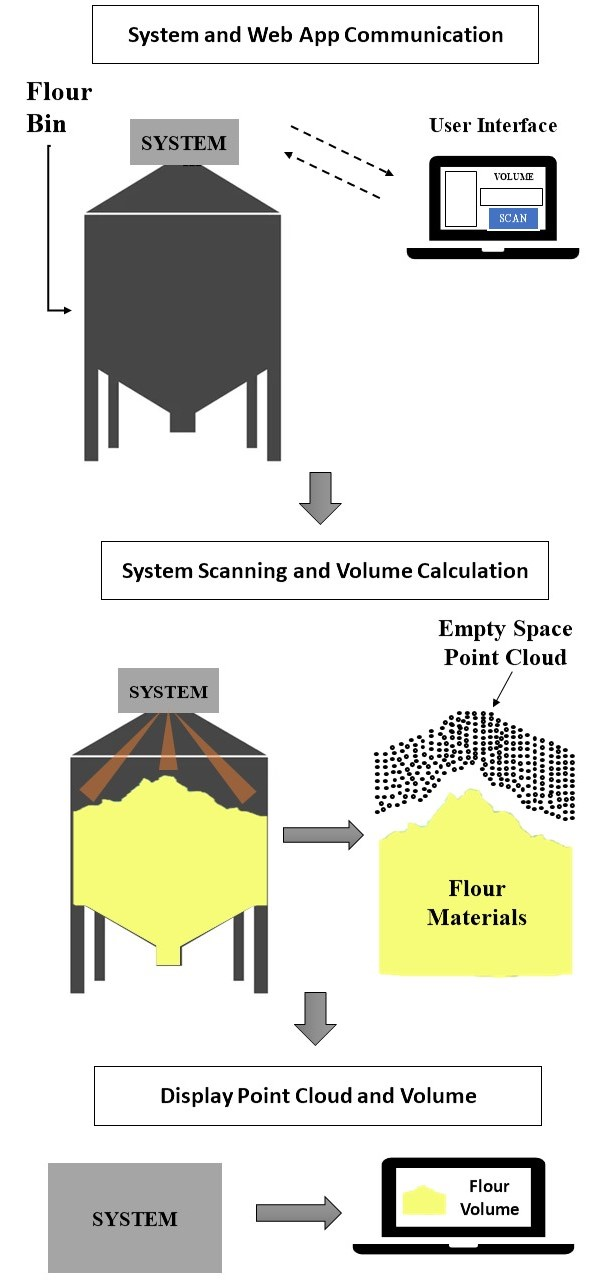
\includegraphics[width=0.6\textwidth, height=1.2\textwidth]{conceptual_framework_diagram.jpg}
	\caption{General Conceptual Flow}
	\label{fig:conceptual-framework}
\end{figure}

\section{Theoretical Framework}
\label{intro:sec:Theoretical Framework}
This section introduces the fundamental theories that guides the underlying principles, methodologies and technologies involved in the study.

\subsection{Calculating Storage Materials Volume using Depth Measurement}
The volume of stored grain is typically calculated using the depth measurement. Once the equivalent level height of the grain is determined based on the depth measurement and surface profile assessment, this height is multiplied by the conversion factor to obtain the volume of the stored grain. This calculation accounts for the headspace between the eave and the grain surface. The underlying calculation with a single and non complex geometric shape can be presented as follows:

\begin{equation}
	V = A \cdot h
\end{equation}

Where:
\begin{align*}
	V & : \text{Volume of the storage container}   \\
	A & : \text{Area of the base of the container} \\
	h & : \text{Height or depth of the container}
\end{align*}

\subsection{3D Polar Coordinate to Cartesian Coordinate}
Converting polar coordinates to cartesian coordinates in three dimensions involves considering the radial distance ($\rho$), the polar angle ($\theta$), and the azimuthal angle ($\phi$). Given a point in spherical coordinates ($\rho$, $\theta$, $\phi$), the corresponding Cartesian coordinates ($x$, $y$, $z$) can be calculated as follows:
\begin{equation}
	x = \rho \cdot \sin(\theta) \cdot \cos(\phi)
\end{equation}
\begin{equation}
	y = \rho \cdot \sin(\theta) \cdot \sin(\phi)
\end{equation}
\begin{equation}
	z = \rho \cdot \cos(\theta)
\end{equation}

Where:
$x$, $y$, and $z$ represent the Cartesian coordinates of the point.
$\rho$ is the radial distance from the origin to the point.
$\theta$ is the polar angle measured from the positive $z$-axis to the point.
$\phi$ is the azimuthal angle measured from the positive $x$-axis to the projection of the point onto the $xy$-plane.

\begin{figure}[H]
	\centering
	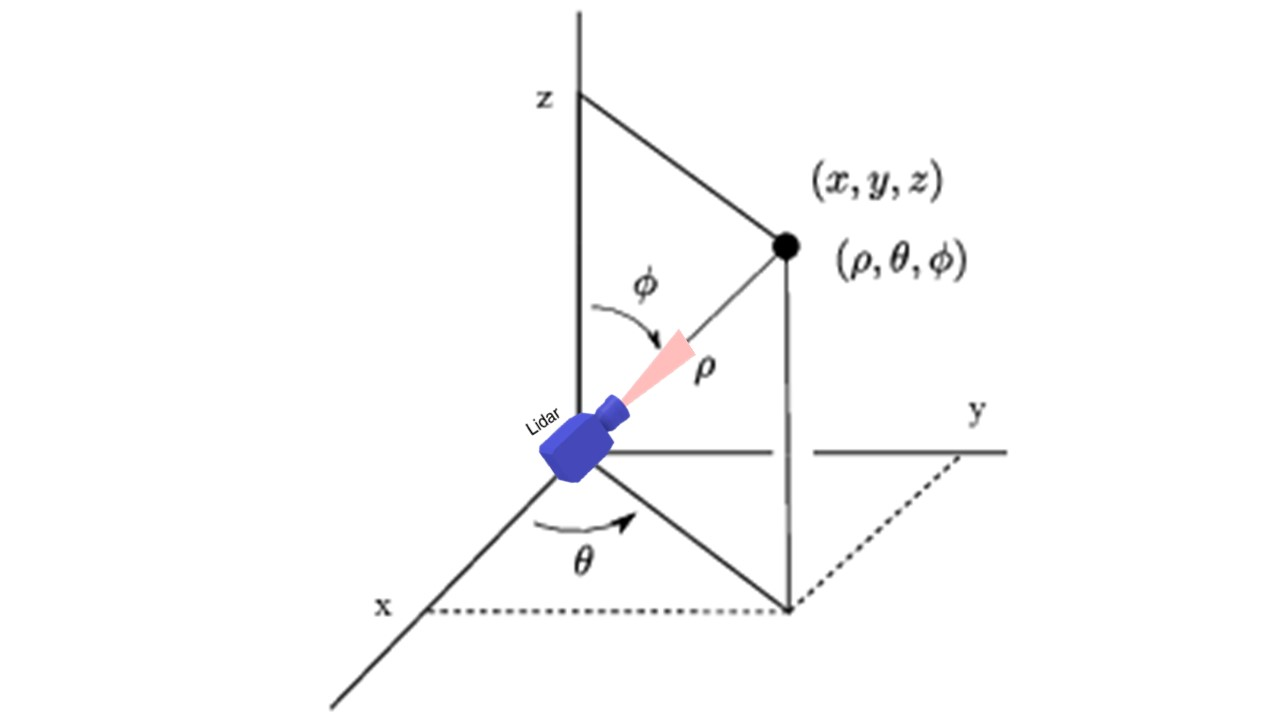
\includegraphics[width=1\textwidth]{Figures/point cloud conversion}
	\caption{LiDAR Scan Range Conversion from Polar Coordintes $(\rho,\theta,\phi)$, to Cartesian Coordinate $(x,y,z)$}
	\label{ch3:fig:point_cloud_conversion}
\end{figure}

\subsection{Point Cloud Data}
A set of points in three dimensions that represent an object's or scene's surface is called a point cloud. Point clouds can be generated through a variety of methods, including photogrammetry, LiDAR, and 3D scanning. Processing and evaluation of these point clouds for a variety of applications is an increasing area of point cloud processing.


\subsection{Computational Geometry using Convex Hull}
The study of the development and evaluation of algorithms for geometric problems in low dimensions—usually two or three—is known as computational geometry. As the smallest convex polygon containing a given set of points, the Convex Hull is a fundamental concept in computational geometry. The convex hull represents the smallest convex set enclosing a given set of points in a Euclidean space as figure \ref{ch1:fig:convex_hull_theory} illustrated. It adheres to principles of convexity, ensuring that the shape remains convex, and minimality, guaranteeing it encompasses the points with minimal expansion.

The Gift Wrapping algorithm, which has a time complexity of O(nh), where n is the number of points and h is the number of points on the hull, is one straightforward method for calculating the Convex Hull.

The equation \ref{ch1:eq:convex_hull} defines the convex hull of a set of points $P_j$ in N-dimensional space. The variable $C$ represents a point in the convex hull, $\lambda_j$ are non-negative weights, and $A_j$ are some constraints. The summation iterates over all points from $j=1$ to $N$.

\begin{equation}
	\label{ch1:eq:convex_hull}
	C = \left\{ \sum_{j=1}^{N} \lambda_j P_j: \lambda_j \geq 0 \text{ for all } j \text{ and } \sum_{j=1}^{N} \lambda_j = 1 \right\}
\end{equation}




\begin{figure}[H]
	\centering
	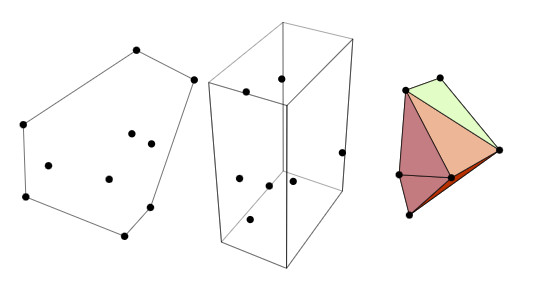
\includegraphics[width=0.8\textwidth]{convex_hull_3d}
	\caption{Convex Hull of Set of Points}
	\label{ch1:fig:convex_hull_theory}
\end{figure}

\subsection{ROS Nodes, Topics, and Subscribe-Publish Relationship}
A framework for building complicated robotic systems that is adaptable is called Robot Operating System (ROS). It makes it possible for nodes, software components that carry out particular functions, to communicate with one another. Topics, also referred to as buses, are the methods by which nodes exchange messages with one another. A key component of ROS is the publish-subscribe connection, in which nodes can publish or subscribe to topics.

Nodes in ROS have the ability to simultaneously subscribe to an indefinite number of topics and share data to an indefinite number of topics. One of the main methods of data communication between nodes, and consequently between other components of the system, is through topics \citep{St-Onge2022}. A node must first advertise a topic before publishing content, or messages, into it in order to exchange information. The first part is completed in the node's initialization code, and the second is completed each time new data has to be shared, usually at a predetermined frequency inside the main loop of the code. Conversely, the node or nodes that need the content of a topic will subscribe to it. The subscriber will associate a callback function triggered for each new incoming message \citep{St-Onge2022}.

%These formulas allow you to convert spherical coordinates to Cartesian coordinates, providing a way to represent points in three-dimensional space using different coordinate systems.


%The research is based on the idea of using automation for industrial operations, specifically in the food industry. Point cloud data is a collection of an unorganized set of x, y, and z coordinates in a three-dimensional space. There are various ways to acquire point cloud data, and one possible way is through active non-contact sensing technology such as LiDAR sensor. LiDAR uses Time-of-Flight (TOF) method of measuring distance between the sensor to the object. TOF scanners are inexpensive compared to other specialized 3D scanners \citep{chua2017}. The researcher will utilize LiDAR to acquire 3D point cloud data because of its ability to gather points data and converts them into a global world coordinate frame \citep{bi2021}. The study does, however, acknowledge the potential limits of LiDAR, when the environment is prone to medium (e.g., water vapor, gases, dust particle, etc.) that can obstruct the target surface, the LiDAR acquired point cloud data that may alter the precision of the data \citep{chua2017}. Thus, the researcher will manage the raw point cloud data by filtering the factoring medium such as dust. Lastly, Delaunay Triangulation is a computational geometry computation that connects a set points to form a mesh of triangles. It can be used for volume estimation by calculating the volume of a convex hull which will be use in this study.

\section{Definition of Terms}
\label{intro:sec:Definition of Terms}

\begin{enumerate}
	\item \textbf{LiDAR} \textemdash stands for Light Detection and Ranging, can also be describe as Light Imaging, Detection, and Ranging. It is a method for determining ranges by targeting an object or a surface with a laser and measuring the time-of-flight to determine the distance.

	\item \textbf{Bin} \textemdash is a large container used to store materials, such as grain, coal, sand, or other bulk goods. They are typically made of metal, plastic, or wood and come in various sizes, shapes, and designs.

	\item \textbf{ROS} \textemdash Robot Operating System is a set of open-source libraries and tools designed to help developers build robot applications. It provides a common framework for creating, managing and sharing code, data, and other resources related to robotic systems.

	\item \textbf{Point Cloud} \textemdash is a set of data points in a three-dimensional space, typically representing the surface of an object. Each point in the cloud is defined by its three-dimensional coordinates (x, y, and z) and may also include additional information such as color, intensity, or normal vector.
	\item \textbf{Convex Hull} \textemdash is the minimum convex polygon from the set of points that encompasses all of the points in the set.

\end{enumerate}